\documentclass[../tesi.tex]{subfiles}
\begin{document}
\chapter{Orchestrazione di Flussi di lavoro}
\begin{figure}[htbp]
  \centering
  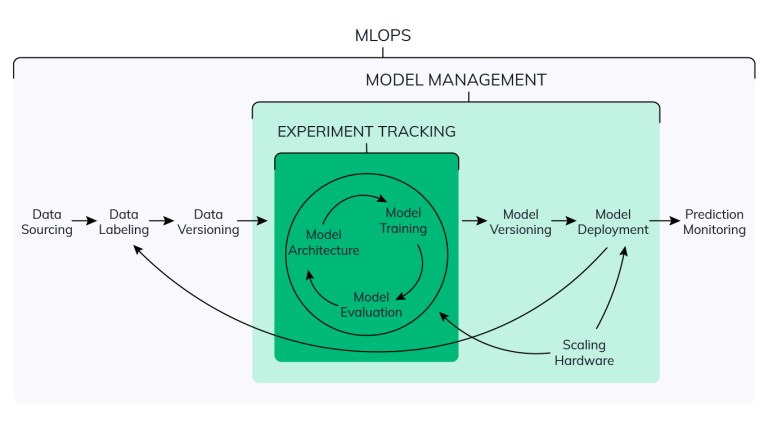
\includegraphics[width=.9\textwidth]{MLops.jpg} 
  \caption{MLops}
  \end{figure}

Dopo aver visto che tra i vari casi di studio troviamo una linea comune nella pipeline di utilizzo del Machine Learning, proviamo automatizzare le invarianti trovate nel capitolo precedente.\\
Negli ultimi anni i ricercatori stanno implementando diversi framework automatici che ci danno la possibilità di automatizzare il flusso di lavoro per la costruzione del modello.\\
Come visto in precedenza intendiamo: raccolta dati, creazione e implementazione del modello e successivamente alla distribuzione permettono la riproduzione e il monitoraggio.\\
Le pipeline ML, inoltre, aiutano a migliorare le prestazioni e la gestione dell'intero modello.
Possiamo semplicemente semplificare lo schema visto in precedenza come segue, lasciando la gestione del modello assegnata al framework.\\
Gli strumenti per l’orchestrazione ML sono usati per automatizzare e gestire i workflow e le infrastrutture delle pipeline con semplici interfacce, aiutando i data scientists e al team di ML di concentrarsi solo sul necessario.\\
Orchestrare un flusso di lavoro è fondamentale per un’azienda che investe nel ML, perciò è necessario capire come automatizzare il maggior numero di risorse, tra cui l’estrazione dell’output del modello con dei monitoraggi costanti durante la fase di produzione.\\
Questi campi che stiamo analizzando sono un sottoinsieme di MLOps: un insieme di pratiche per la collaborazione e la comunicazione tra data scientist e professionisti delle operazioni. Applicando queste tecniche pratiche aumenta la qualità finale, semplifica il processo di gestione e automatizza l’implementazione di modelli di ML e DL in ambienti di produzione su larga scala(schema sottostante)

  \section{Framework}
  Prima di elencare una lista di tools di gestori di risorse di ML, diventa necessario anticipare una distinzione tra un software in fase di ricerca e un software giá a livello di produzione ovvero giá utilizzato a livello aziendale.\\
  Un software ancora in fase di ricerca, spesso utilizzato a livello accademico, offre delle funzionalitá magari non ancora rilasciate nel mondo ``Aziendlae'' avendo delle "particolaritá" che altri software magari \textit{"in produzione"} non possiedono.\\
  Questi ultimi, a loro volta, si differenziano grazie a caratteristiche quali l'affidabilitá.  
  \subsection{ZenML} 
  ZenML è uno strumento open-source per operazione di ML.
  Lo strumento si focalizza sui problemi di riproduzioni basati sulla produzione, come le difficoltà di versioning e modelli, organizzazione di workflow di ML e la distribuzione. Può lavorare a fianco a un altro strumento di orchestrazione dei flussi di lavoro per fornire un semplice percorso per rilasciare il modello ML in produzione.\\
  È possibile verificare con precisione dati, modelli e configurazioni. Ti consente di valutare in maniera semi-automatica il modello, confrontare le pipeline di addestramento e distribuire la preelaborazione nel cloud.
  
  \begin{figure}[htbp]
    \centering
    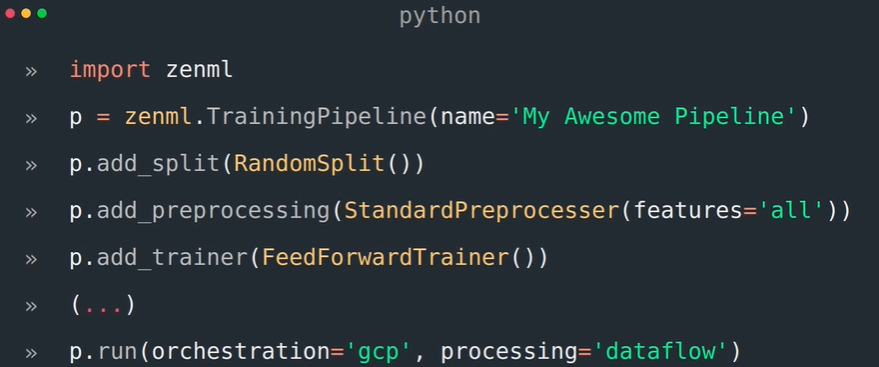
\includegraphics[width=.9\textwidth]{zenML.png} 
    \caption{ZenML}
    \end{figure}
  Come vediamo dalla figura 4.2 ogni metodo implementa uno specifico passaggio del workflow, vincolando i passaggi da eseguire sul modello a discrezione del Framework stesso; se l'addestramento (\textit{add\textunderscore trainer}) appare prima del processamento dei dati (\textit{add\textunderscore preprocessing}), sará compito del framework nel metodo (\textit{run}) organizzare l'ordine delle operazioni da eseguire nel modello.
  
  \subsection{Kedro}
Kedro é uno strumento open-source di orchestrazione basato su Python, che permette di creare workflow per ML riproducibili, mantenibili e modulari, semplificando i processi e rendendoli più accurati.\\
Kedro integra l’ingegneria del software in un ambiente di apprendimento automatico, con concetti quali: modularità, divisione degli interessi e versioning.\\
Astraendo la pipeline, è possibile automatizzare le dipendenze tra il codice Python e la visualizzazione del Workflow. L’obiettivo principale è la creazione di codice di data science gestibile per affrontare le carenze di Jupiter(applicazione web open-source, utile per condividere documenti che contengono codice live, equazioni e grafi ecc.)\\
Questo strumento crea un lavoro di squadra più semplice a vari livelli, e fornisce un efficiente ambiente di coding con codice modulare e riusabile.
\begin{figure}[htbp]
  \centering
  \includegraphics[width=.9\textwidth]{KedroPipeline.png} 
  \caption{Kedro}
  \end{figure}  
\subsection{Flyte}
Flyte è uno strumento open-source di alta fascia che permette di facilitare la creazione di flussi di lavoro del ML. È una piattaforma di programmazione ad elaborazione distribuita e strutturata, con flussi di lavoro concorrenti, scalabili e mantenibili per l’apprendimento automatico e l’elaborazione dei dati.\\
Flyte gestisce già più di dieci mila workflow, è basato su Kubernetes e offre portabilità, scalabilità e affidabilità.\\
L’interfaccia è elastica, intuitiva e facile da usare; offre inoltre parametri, linee di dati e caching per organizzare i workflow.\\
L’intera piattaforma è dinamica ed estensibile attraverso vari plug-in per assistere la creazione e l’implementazione dei vari workflow. Tali Workflow, a loro volta, possono essere reiterati, annullati, sperimentati e condivisi per accelerare il processo di sviluppo dell’intero team.\\
Poiché ogni entità in Flyte è immutabile, insieme a ogni modifica esplicita assunta come nuova versione, diventa semplice ed efficiente iterare, sperimentare e tornare indietro nei Workflow.
\begin{figure}[htbp]
  \centering
  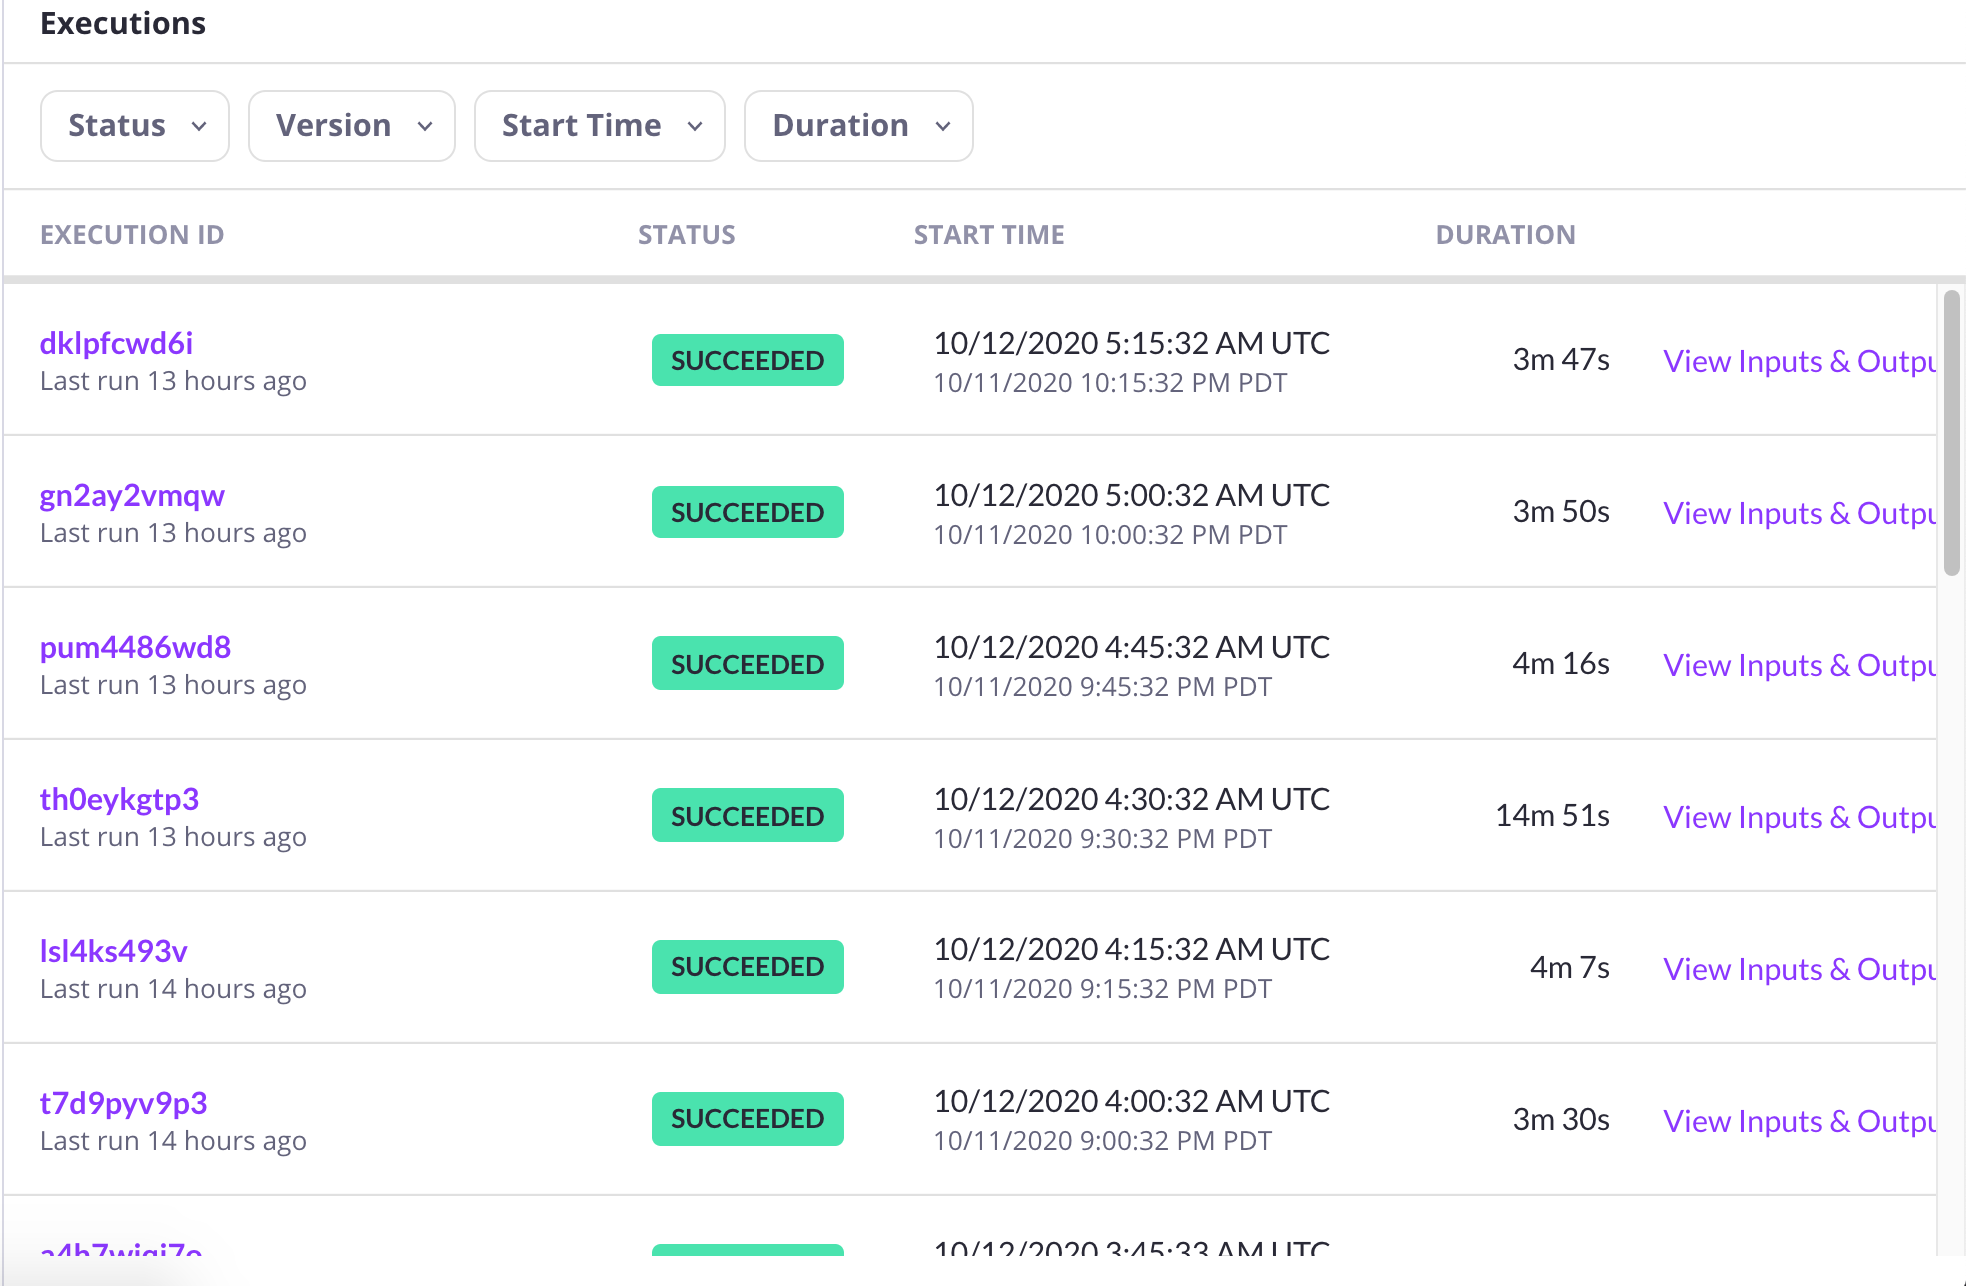
\includegraphics[width=.9\textwidth]{Flyte.png} 
  \caption{Flyte Console}
  \end{figure}

  \newglossaryentry{server-less}{name={Server-Less},description={Il ServerLess computing é un modello di sviluppo Cloud Native che consente agli sviluppatori di creare ed eseguire applicazioni senza gestire i server, i quali saranno astratti dallo sviluppo dell'app. La gestione delle risorse, la manutenzione e la scalabilitá del server saranno tutti compiti affidati al provider dei servizi cloud. }}
  \newglossaryentry{Microservizi}{name={Microservizi},description={I Microservizi sono un approccio particolare alla realizzazione di applicazioni. Una applicazione diventa un insieme di servizi, i quali possono essere compilati e implementati in maniera indipendente. Inoltre ogni Microservizio puó funzionare, o meno, senza compromettere gli altri.}}
\newglossaryentry{grafo aciclico}{name={Grafo Aciclico},description={Un grafo aciclico é un particolare tipo di grafo in cui non sono presenti cicli.}}
  
\subsection{MLRun}
MLRun è uno strumento open-source di orchestrazione di orchestrazione di workflow/pipeline. Ha integrato un approccio per organizzare pipeline di ML, a partire dallo sviluppo iniziale, costruzione del modello verso tutti processi che portano allo sviluppo in produzione.\\
Esso integra un vasto reparto di strumenti e plugin per lavorare con caratteristiche e modelli insieme alla distribuzione del flusso di lavoro.\\
MLRun dispone di un archivio di funzionalità e artefatti per controllare l’inserimento, l’elaborazione e l’archiviazione dei dati su più repository e con tecnologie diverse.\\
È un elastico servizio ``\Gls{server-less}'' per convertire semplice codice in scalabili e organizzati ``\Gls{Microservizi}''; diventa così più semplice e leggero fare esperimenti, allenare i modelli e testarli, e implementare dei flussi di lavoro della pipeline in tempo reale.\\
L’interfaccia utente complessiva ha una struttura centralizzata per gestire flussi di lavoro di ML. Le caratteristiche principali includono una rapida implementazione, elastica scalabilità, gestione delle funzionalità e un usabilità flessibile.\\


\subsection{Couler}
Couler ha un’interfaccia unificata per il codice e la gestione dei flussi di lavoro con differenti motori e framework di workflow.\\
L'unico strumento di orchestrazione del flusso di lavoro per la gestione di altri strumenti di orchestrazione.\\
Anch’esso è open-source e a differenza di altri motori, che hanno complessi livelli di astrazione, l’interfaccia di Couler rende estremamente semplice la gestione di questi livelli.\\
Couler ha uno stile di programmazione imperativo per la definizione del workflow integrato però con un supporto per la costruzione automatica di un \Gls{grafo aciclico}.\\
I Servizi di Couler sono altamente estendibili, supportando altri motori di flussi di lavoro.\\
Facilita l’addestramento dei modelli di ML, aumentando la modularità e la riusabilità.

\section{Conclusioni}

\end{document}